\documentclass[10pt,a4paper]{article}
\usepackage[margin=0.7in]{geometry}
\usepackage{multicol}
\usepackage{amsmath}
\usepackage{tikz}
\usepackage{enumitem}
\usepackage{titlesec}
\usepackage{booktabs}
\usepackage{fontspec}

% Compact formatting
\setlength{\columnsep}{0.7cm}
\setlength{\parindent}{0pt}
\setlength{\parskip}{0.12cm}
\titlespacing{\section}{0pt}{0.4cm}{0.15cm}
\titlespacing{\subsection}{0pt}{0.25cm}{0.08cm}
\titlespacing{\subsubsection}{0pt}{0.2cm}{0.05cm}

% Custom section style
\titleformat{\section}{\large\bfseries}{}{0em}{}
\titleformat{\subsection}{\normalsize\bfseries}{}{0em}{}
\titleformat{\subsubsection}{\normalsize\bfseries\itshape}{}{0em}{}

\begin{document}

\begin{center}
{\LARGE \textbf{Production and Cost}}\\[0.15cm]
{\normalsize \textit{Topic 6: Theory of the Firm -- Output, Inputs, and Cost Curves}}\\[0.15cm]
\hrule
\end{center}
\vspace{-0.3cm}

\begin{multicols}{2}
\footnotesize

% ============================================================================
% PART 1: DEFINITIONS AND CORE CONCEPTS
% ============================================================================
\section*{1. Core Definitions}

\subsection*{Production Function}
A \textbf{Production Function} expresses the \textbf{technological relationship} between physical inputs (factors of production) and the maximum physical output obtainable, given the current state of technology.

\[
Q = f(L, K, N, E, \dots)
\]
Where: $Q$ = Total product/output; $L$ = Labor; $K$ = Capital; $N$ = Land/Natural resources; $E$ = Entrepreneurship.

\textbf{Key Properties:}
\begin{itemize}[leftmargin=*,nosep]
    \item \textbf{Technical Efficiency:} Gives \textit{maximum} output for given inputs (no waste).
    \item \textbf{Flow Concept:} Output is measured per unit of time.
    \item \textbf{Technology-Specific:} A change in technology shifts the function.
    \item \textbf{Specifies Factor Proportions:} How inputs combine (complements vs. substitutes).
\end{itemize}

\subsection*{Factors of Production: Fixed vs. Variable}
The distinction is based on the \textbf{time horizon}:
\begin{itemize}[leftmargin=*,nosep]
    \item \textbf{Fixed Factors:} Cannot be changed in the \textbf{short run} (e.g., factory building, heavy machinery, land). Their quantity remains constant regardless of output level.
    \item \textbf{Variable Factors:} Can be adjusted in the short run (e.g., labor, raw materials, electricity). Their quantity varies directly with output.
    \item \textbf{Short Run:} At least one factor is fixed. The firm operates within a given ``scale'' of plant. $Q = f(L, \bar{K})$.
    \item \textbf{Long Run:} All factors are variable. The firm can change its scale of operations. No fixed factors. $Q = f(L, K)$ -- both variable.
\end{itemize}

% ============================================================================
% PART 2: HOW TO REMEMBER
% ============================================================================
\section*{2. Memory Triggers and Conceptual Anchors}

\begin{itemize}[leftmargin=*,nosep]
    \item \textbf{Production Function = Recipe:} Inputs (ingredients) $\to$ Output (cake). Technology = cooking method. Better tech = more cake from same ingredients.
    \item \textbf{Fixed vs Variable = ``Can I change it this month?'':} Fixed = ``Stuck with it'' (lease, building). Variable = ``I can hire/fire or buy more'' (workers, materials). Mnemonic: \textbf{S}hort run = \textbf{S}tuck with some factors.
    \item \textbf{Total Product (TP) = Total Output.} Marginal Product (MP) = \textbf{Extra} output from \textbf{one more} unit of variable input. (M for Marginal = More input.)
    \item \textbf{MP and AP Relationship:}
    \begin{itemize}[nosep]
        \item If $MP > AP$, AP is \textbf{rising} (a high marginal student raises the class average).
        \item If $MP < AP$, AP is \textbf{falling} (a low marginal student lowers the average).
        \item $MP$ intersects $AP$ at the \textbf{maximum} of $AP$.
    \end{itemize}
    \item \textbf{Law of Diminishing Returns = Too Many Cooks in the Kitchen:} Adding more and more workers to a fixed kitchen increases total meals initially, but eventually each extra worker adds less (and may even reduce output). Mnemonic: ``Crowding kills productivity.''
    \item \textbf{Returns to Scale = Double the Recipe:}
    \begin{itemize}[nosep]
        \item Double all inputs, output \textbf{more than doubles} = \textbf{Increasing Returns to Scale (IRS)}. (Bulk buying, specialization.)
        \item Double all inputs, output \textbf{exactly doubles} = \textbf{Constant Returns to Scale (CRS)}.
        \item Double all inputs, output \textbf{less than doubles} = \textbf{Decreasing Returns to Scale (DRS)}. (Management complexity.)
    \end{itemize}
    \item \textbf{Cost Curves -- Shape Memory:}
    \begin{itemize}[nosep]
        \item \textbf{TC} starts positive (due to fixed cost) and rises.
        \item \textbf{MC, AVC, ATC} are \textbf{U-shaped}: First fall due to specialization/returns, then rise due to diminishing returns.
        \item \textbf{AFC} always falls (spreading overhead over more units).
        \item \textbf{MC} cuts \textbf{AVC} and \textbf{ATC} at their \textbf{minimum points}. (If marginal is below average, average falls; if above, average rises.)
    \end{itemize}
    \item \textbf{Short Run vs. Long Run Cost:} LR cost curve is the \textbf{envelope} of SR cost curves. In the LR, you can choose the optimal plant size for each output level.
\end{itemize}

% ============================================================================
% PART 3: MATHEMATICAL FRAMEWORK
% ============================================================================
\section*{3. Product Concepts \& Formulas}

\subsection*{Total, Average, and Marginal Product}
Let $Q = f(L, \bar{K})$ be the short-run production function with Labor ($L$) as the variable factor.

\textbf{Total Product of Labor ($TP_L$):} $TP_L = Q = f(L, \bar{K})$.

\textbf{Average Product of Labor ($AP_L$):}
\[
AP_L = \frac{TP_L}{L} = \frac{Q}{L}
\]
Measures output per unit of labor (productivity).

\textbf{Marginal Product of Labor ($MP_L$):}
\[
MP_L = \frac{\Delta TP_L}{\Delta L} \quad \text{or} \quad MP_L = \frac{\partial Q}{\partial L}
\]
Additional output from one more unit of labor.

\subsection*{The Law of Diminishing Marginal Returns (Diminishing MP)}
As more units of a \textbf{variable input} are added to a \textbf{fixed input}, eventually the \textbf{marginal product} of the variable input \textbf{declines}, \textit{ceteris paribus}.
\[
\frac{\partial (MP_L)}{\partial L} = \frac{\partial^2 Q}{\partial L^2} < 0 \quad \text{(after some point)}
\]

\textbf{Three Stages of Production (Short-Run):}
\begin{enumerate}[leftmargin=*,nosep]
    \item \textbf{Stage I ($AP_L$ rising):} $MP_L > AP_L$. Increasing average returns. Fixed factors underutilized. \textit{Rational producer won't stop here} (can increase AP by adding more L).
    \item \textbf{Stage II ($AP_L$ falling, $MP_L > 0$):} $MP_L < AP_L$, but $MP_L > 0$. TP still rising. \textbf{This is the rational production range.}
    \item \textbf{Stage III ($MP_L < 0$):} Total product falls. Too many workers relative to fixed capital; negative returns. \textit{Irrational to operate here.}
\end{enumerate}

\subsection*{Returns to Scale (Long-Run Concept)}
When \textbf{all} inputs increase by the same proportion $\lambda > 1$, how does output change?
\[
Q = f(L, K) \quad \Rightarrow \quad \text{Measure } f(\lambda L, \lambda K)
\]
\begin{itemize}[leftmargin=*,nosep]
    \item \textbf{Increasing Returns to Scale (IRS):} $f(\lambda L, \lambda K) > \lambda f(L, K)$ $\Rightarrow$ Output increases more than proportionately.
    \item \textbf{Constant Returns to Scale (CRS):} $f(\lambda L, \lambda K) = \lambda f(L, K)$ $\Rightarrow$ Output increases exactly proportionately. Function is \textbf{homogeneous of degree 1}.
    \item \textbf{Decreasing Returns to Scale (DRS):} $f(\lambda L, \lambda K) < \lambda f(L, K)$ $\Rightarrow$ Output increases less than proportionately.
\end{itemize}

\textbf{Typical Production Function (Cobb-Douglas):}
\[
Q = A L^\alpha K^\beta
\]
Returns to scale: $\alpha + \beta$.
\begin{itemize}[nosep]
    \item $\alpha + \beta > 1 \Rightarrow$ IRS.
    \item $\alpha + \beta = 1 \Rightarrow$ CRS.
    \item $\alpha + \beta < 1 \Rightarrow$ DRS.
\end{itemize}

\textbf{Causes:} IRS due to specialization, indivisibilities, dimensional factors. DRS due to management complexity, coordination problems (``diseconomies of scale'').

\subsection*{Cost Concepts \& Formulas}
\textbf{Total Costs:}
\[
TC = TFC + TVC
\]
\begin{itemize}[nosep]
    \item \textbf{Total Fixed Cost (TFC):} Cost of fixed factors; does not vary with output. (e.g., rent, insurance).
    \item \textbf{Total Variable Cost (TVC):} Cost of variable factors; varies directly with output. (e.g., wages, raw material). $TVC = w \cdot L(Q)$.
\end{itemize}

\textbf{Average Costs:}
\[
AFC = \frac{TFC}{Q}; \quad AVC = \frac{TVC}{Q}; \quad ATC = \frac{TC}{Q} = AFC + AVC
\]

\textbf{Marginal Cost ($MC$):}
\[
MC = \frac{\Delta TC}{\Delta Q} = \frac{\Delta TVC}{\Delta Q} \quad \text{(since TFC constant)}
\]
\[
MC = \frac{w}{MP_L} \quad \text{(Derived: } MC = \frac{d(TVC)}{dQ} = \frac{w \cdot dL}{dQ} = \frac{w}{MP_L}\text{)}
\]
\textbf{Inverse relationship:} When $MP_L$ is rising, $MC$ is falling; when $MP_L$ falls (diminishing returns), $MC$ rises. The U-shape of MC mirrors the inverted-U of MP.

\subsection*{Short-Run vs. Long-Run Cost Curves}
\begin{itemize}[leftmargin=*,nosep]
    \item \textbf{Short-Run Average Cost (SRAC):} U-shaped due to fixed factor constraint; diminishing returns eventually raise AVC and ATC.
    \item \textbf{Long-Run Average Cost (LRAC):} \textbf{Envelope curve} of all possible SRAC curves (each SRAC corresponds to a different plant size). LRAC is typically U-shaped due to economies/diseconomies of scale.
    \item In LR, all factors variable; firm chooses optimal plant size for each output level. LRAC touches each SRAC at the minimum-cost point for that output level (tangency, not necessarily minimum of each SRAC).
\end{itemize}

% ============================================================================
% PART 4: GRAPHICAL ANALYSIS
% ============================================================================
\section*{4. Graphical Illustrations}

\subsection*{TP, AP, and MP Curves \& Stages of Production}
\begin{center}
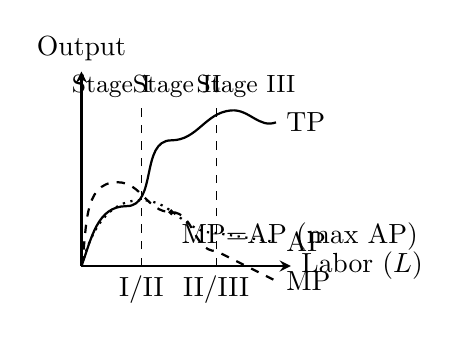
\begin{tikzpicture}[scale=0.38, thick, >=stealth]
    \draw[->] (0,0) -- (7,0) node[right] {Labor ($L$)};
    \draw[->] (0,0) -- (0,6.5) node[above] {Output};
    % TP Curve (sigmoid)
    \draw[thick] (0,0) to[out=70,in=180] (1.5,2) to[out=0,in=180] (3,4.2) to[out=0,in=185] (5,5.2) to[out=5,in=200] (6.5,4.8) node[right] {TP};
    % MP Curve
    \draw[thick, dashed] (0,0) to[out=80,in=180] (1.2,2.8) to[out=0,in=180] (3,1.8) to[out=0,in=180] (4.5,0.5) -- (6.5,-0.5) node[right] {MP};
    % AP Curve
    \draw[thick, dotted] (0,0) to[out=75,in=180] (2,2.2) to[out=0,in=180] (4.5,1.1) -- (6.5,0.8) node[right] {AP};
    % Stage divisions
    \draw[dashed, thin] (2,0) node[below] {I/II} -- (2,5.5);
    \draw[dashed, thin] (4.5,0) node[below] {II/III} -- (4.5,5.5);
    \node at (1,6) {\small Stage I};
    \node at (3.2,6) {\small Stage II};
    \node at (5.5,6) {\small Stage III};
    % MP=AP intersection
    \filldraw (3,1.8) circle (1.5pt) node[below right] {MP=AP (max AP)};
\end{tikzpicture}
\end{center}

\subsection*{Short-Run Cost Curves (Family of Curves)}
\begin{center}
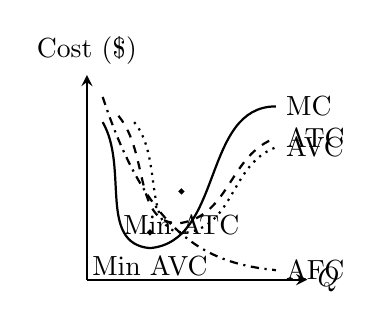
\begin{tikzpicture}[scale=0.4, thick, >=stealth]
    \draw[->] (0,0) -- (7,0) node[right] {$Q$};
    \draw[->] (0,0) -- (0,6.5) node[above] {Cost (\$)};
    % MC
    \draw[thick] (0.5,5) to[out=300,in=175] (2,1) to[out=5,in=180] (6,5.5) node[right] {MC};
    % ATC
    \draw[thick, dashed] (1,5.2) to[out=310,in=185] (3,1.8) to[out=10,in=200] (6,4.5) node[right] {ATC};
    % AVC
    \draw[thick, dotted] (1.5,5) to[out=310,in=185] (3.2,1.5) to[out=10,in=200] (6,4.2) node[right] {AVC};
    % AFC
    \draw[thick, dashdotted] (0.5,5.8) .. controls (2,1.2) and (4,0.5) .. (6,0.3) node[right] {AFC};
    % Intersection points
    \filldraw (2,1.5) circle (1.5pt) node[below=5pt] {Min AVC};
    \filldraw (3,2.8) circle (1.5pt) node[below=5pt] {Min ATC};
\end{tikzpicture}
\end{center}
\textit{Note: MC intersects AVC and ATC at their respective minimum points. ATC = AVC + AFC. The vertical gap between ATC and AVC shrinks as AFC declines.}

\subsection*{Long-Run Average Cost (LRAC) as Envelope}
\begin{center}
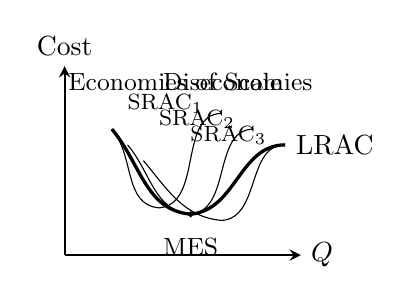
\begin{tikzpicture}[scale=0.4, thick, >=stealth]
    \draw[->] (0,0) -- (7.5,0) node[right] {$Q$};
    \draw[->] (0,0) -- (0,6) node[above] {Cost};
    % SRAC curves
    \draw[thin] (1.5,4) to[out=310,in=175] (3,1.5) to[out=5,in=180] (5,4.5);
    \draw[thin] (2,3.5) to[out=310,in=175] (4,1.3) to[out=5,in=180] (6,4);
    \draw[thin] (2.5,3) to[out=310,in=175] (5,1.1) to[out=5,in=180] (7,3.5);
    \node at (3.2,4.8) {\footnotesize SRAC$_1$}; \node at (4.2,4.3) {\footnotesize SRAC$_2$}; \node at (5.2,3.8) {\footnotesize SRAC$_3$};
    % LRAC envelope
    \draw[very thick] (1.5,4) to[out=310,in=175] (4,1.3) to[out=5,in=180] (7,3.5) node[right] {LRAC};
    \node at (3.5,5.5) {\small Economies of Scale};
    \node at (5.5,5.5) {\small Diseconomies};
    \filldraw (4,1.3) circle (1.5pt) node[below=5pt] {\small MES};
\end{tikzpicture}
\end{center}
\textit{LRAC is the lower envelope of all SRAC curves. Minimum Efficient Scale (MES) is the lowest output level at which LRAC is minimized.}

\columnbreak

% ============================================================================
% PART 5: DETAILED RELATIONSHIPS
% ============================================================================
\section*{5. Key Relationships and Derivations}

\subsection*{Product-Cost Duality}
There is a \textbf{mathematical duality} between production and cost:
\begin{itemize}[leftmargin=*,nosep]
    \item \textbf{MC and MP:} $MC = \frac{w}{MP_L}$. When MP is high (Stage I), MC is low. When diminishing returns set in (MP falls, Stage II), MC rises.
    \item \textbf{AVC and AP:} $AVC = \frac{w \cdot L}{Q} = \frac{w}{AP_L}$. When AP is high, AVC is low. AVC falls when AP rises, and rises when AP falls. AVC reaches minimum at maximum AP.
    \item \textbf{Shape connection:} The U-shape of MC and AVC is derived directly from the inverted-U shape of MP and AP, respectively.
\end{itemize}

\subsection*{Why MC Intersects AVC and ATC at Minimum}
\textbf{Mathematical Proof:} At the minimum of AVC, $\frac{d(AVC)}{dQ} = 0$.
\[
AVC = \frac{TVC}{Q} \quad \Rightarrow \quad \frac{d(AVC)}{dQ} = \frac{Q \cdot \frac{d(TVC)}{dQ} - TVC \cdot 1}{Q^2} = \frac{Q \cdot MC - TVC}{Q^2}
\]
Setting derivative = 0: $Q \cdot MC = TVC \Rightarrow MC = \frac{TVC}{Q} = AVC$.

Similarly, at min ATC: $MC = ATC$. This is \textbf{essential for cost-curve diagram accuracy}.

\subsection*{Long-Run Cost Minimization}
In the long run, the firm chooses $L$ and $K$ to minimize cost for a given output $\bar{Q}$:
\[
\min \; wL + rK \quad \text{s.t.} \quad f(L, K) = \bar{Q}
\]
Condition: $MRTS_{LK} = \frac{MP_L}{MP_K} = \frac{w}{r}$.
Cost function: $C(Q) = wL^*(w,r,Q) + rK^*(w,r,Q)$.

\subsection*{Economies and Diseconomies of Scale}
\begin{itemize}[leftmargin=*,nosep]
    \item \textbf{Economies of Scale (falling LRAC):} Caused by \textbf{specialization of labor/management}, \textbf{indivisibilities} of capital (large machines more efficient), \textbf{volume discounts} on inputs, \textbf{learning by doing}, \textbf{by-product utilization}.
    \item \textbf{Diseconomies of Scale (rising LRAC):} Caused by \textbf{management complexity}, \textbf{communication breakdowns}, \textbf{alienation of labor}, \textbf{increased bureaucracy}, \textbf{transportation costs} as the firm grows geographically.
    \item \textbf{Constant Returns to Scale (flat LRAC):} Perfect scalability; firm can replicate operations efficiently.
\end{itemize}

% ============================================================================
% PART 6: EXTENSIVE CASE STUDIES
% ============================================================================
\section*{6. Comprehensive Case Studies}

\subsection*{Case Study 1: Henry Ford's Assembly Line and the Law of Diminishing Returns}

\textbf{Background:} In 1913, Henry Ford revolutionized automobile manufacturing by introducing the \textbf{moving assembly line} at the Highland Park plant in Michigan. Prior to this, cars were handcrafted by skilled workers. The assembly line broke production into specialized, repetitive tasks, dramatically increasing productivity and reducing costs. The Model T price fell from \$850 (1908) to under \$300 (1924), making the automobile a mass-market product.

\textbf{Production Function Analysis:}
\begin{itemize}[leftmargin=*,nosep]
    \item \textbf{Short-run:} Capital (assembly line, factory) was fixed. Labor was variable.
    \item \textbf{Initial phase (Stage I and early Stage II):} Adding workers to the fixed assembly line led to \textbf{increasing marginal returns}. With specialization, workers became faster at their single repeated task. The division of labor raised $MP_L$. Total product rose sharply, and $AP_L$ (output per worker) increased.
    \item \textbf{Optimal point:} Ford's $5-a-day wage policy (double the prevailing wage) reduced turnover and absenteeism, keeping the labor force stable and productive. The plant operated near the boundary of Stage I and Stage II, where $MP_L \approx AP_L$, maximizing labor productivity.
\end{itemize}

\textbf{The Diminishing Returns Test:}
In later years, Ford attempted to push the system further by continuously speeding up the assembly line and adding more workers to the same physical plant. At some point, diminishing returns set in:
\begin{itemize}[leftmargin=*,nosep]
    \item Workers became \textbf{overcrowded} on the line; task spaces were physically constrained.
    \item Fatigue increased; error rates and accidents rose.
    \item The marginal product of an additional worker became very low; too many workers per machine caused idle time and interference.
    \item Total product still grew, but at a diminishing rate (Stage II). Eventually, adding more workers could have led to negative marginal product (Stage III) -- workers literally getting in each other's way.
\end{itemize}

\textbf{Cost Implications:}
\begin{itemize}[leftmargin=*,nosep]
    \item Initially, high $MP_L$ meant low $MC$ ($MC = w/MP_L$). The \$5 wage was easily absorbed by the massive productivity gains.
    \item As diminishing returns set in, $MP_L$ fell, and $MC$ began to rise. AVC also started increasing after the point of maximum AP.
    \item Ford eventually had to build entirely new, larger plants (e.g., River Rouge Complex, completed 1928) because the existing fixed capital (Highland Park) constrained further output expansion. This was the \textbf{transition from Short Run to Long Run} -- scaling up all inputs to escape the constraints of the fixed factor.
\end{itemize}

\textbf{The River Rouge Complex -- Economies of Scale (Long-Run):}
The River Rouge plant was the largest integrated factory in the world. It demonstrated massive \textbf{internal economies of scale}:
\begin{itemize}[leftmargin=*,nosep]
    \item \textbf{Vertical Integration:} Raw materials (iron ore, coal) arrived at one end; finished Model A cars drove out the other end.
    \item \textbf{Technical Economies:} Specialized machinery for each component (engine blocks, chassis, glass), achieving very low unit costs.
    \item \textbf{Labor Specialization:} Over 100,000 workers, each highly specialized.
    \item \textbf{By-product Use:} Slag from steel production was sold; waste heat reused.
\end{itemize}
However, as the plant grew even larger, \textbf{diseconomies of scale} emerged:
\begin{itemize}[leftmargin=*,nosep]
    \item Management coordination became extremely complex; bureaucratic layers multiplied.
    \item Labor relations deteriorated; the massive workforce was difficult to manage, leading to the famous 1937 ``Battle of the Overpass'' union clashes.
    \item Communication and scheduling across the huge site became inefficient.
    \item LRAC likely began to rise at very large output scales.
\end{itemize}

\textbf{Economic Lessons:}
\begin{enumerate}[leftmargin=*,nosep]
    \item The \textbf{short-run production function} with diminishing returns explains both early productivity miracles and eventual constraints within a given plant.
    \item The \textbf{transition from SR to LR} is a strategic decision: when diminishing returns make MC rise too high, the firm expands fixed capital.
    \item \textbf{Economies of scale} drive long-run cost reductions, but \textbf{diseconomies of scale} eventually limit firm size. Ford's trajectory illustrates both sides of the U-shaped LRAC curve.
    \item The relationship $MC = w/MP_L$ directly links worker productivity to marginal cost -- the fundamental driver of pricing and profitability.
\end{enumerate}

\subsection*{Case Study 2: Semiconductor Fabrication -- Returns to Scale and the Cost Race (TSMC vs. Intel)}

\textbf{Background:} Semiconductor manufacturing (chip fabrication, or ``fabs'') is one of the most capital-intensive industries in the world. A single state-of-the-art fabrication plant costs \$10--\$20 billion. The industry is characterized by massive \textbf{economies of scale}, a steep \textbf{learning curve}, and intense competition driven by cost-per-transistor reduction. Taiwan Semiconductor Manufacturing Company (TSMC) has become the world's dominant player by focusing solely on manufacturing (a ``pure-play foundry''), while Intel historically combined design and manufacturing (IDM model).

\textbf{Production Function:}
The output of a fab can be modeled as a function of capital-intensive equipment (lithography machines, etchers) and highly skilled labor.
\[
Q = f(K, L) \quad \text{with significant fixed capital } K \text{ (ASML EUV machines cost \$200M+ each)}
\]

\textbf{Short-Run Production:}
\begin{itemize}[leftmargin=*,nosep]
    \item \textbf{Fixed Factor:} The fab building and installed equipment ($K$ fixed). Expanding output requires running the fab at higher capacity utilization rates, adding shifts, overtime ($L$ variable).
    \item \textbf{Initially:} MP of labor may rise as the workforce gets trained and processes are optimized (learning-by-doing within a shift).
    \item \textbf{Eventually:} Diminishing returns hit. Adding extra shifts (nights, weekends) leads to worker fatigue, increased defect rates, equipment downtime, and maintenance constraints. The marginal wafer output from an extra labor hour declines. Running fabs above 90--95\% capacity utilization becomes inefficient ($MC$ rises sharply due to defects and breakdowns).
\end{itemize}

\textbf{Long-Run Returns to Scale:}
When Intel or TSMC build a new fab (increasing $K$ and $L$ proportionately), they experience significant economies of scale:

\begin{enumerate}[leftmargin=*,nosep]
    \item \textbf{Technical Indivisibilities:} An EUV lithography machine produces wafers at a massive minimum scale. A larger fab better utilizes the high fixed cost of these machines. \textbf{Doubling fab size more than doubles output} because the most expensive tools operate more efficiently.
    \item \textbf{Learning and Experience Curve:} Cumulative output drives down defect densities and improves yield (the percentage of functional chips per wafer). TSMC's cumulative output is enormous, giving it a cost advantage Intel struggles to match. \textit{Yield improvement} is a pure economy of scale -- fixed R\&D and learning costs spread over larger volume.
    \item \textbf{Economies of Scope:} Advanced fabs can produce multiple chip designs for different clients, sharing the massive fixed costs across many products. TSMC's pure-play model amplifies this -- it serves hundreds of clients (Apple, AMD, Nvidia) on the same process technology.
    \item \textbf{R\&D Amortization:} Semiconductor process R\&D costs billions per node (e.g., moving from 7nm to 5nm technology). These costs are fixed regardless of how many chips are eventually produced. TSMC's large volume allows it to amortize R\&D across a far greater number of chips than Intel, lowering \textbf{average fixed cost (AFC)} dramatically.
\end{enumerate}

\textbf{The Cost Race -- Why Size Matters:}
The average cost per transistor has fallen exponentially (Moore's Law), but the cost per fab has risen exponentially (Rock's Law). This creates a \textbf{virtuous cycle} of scale for the leader:
\begin{itemize}[leftmargin=*,nosep]
    \item Larger volume $\to$ lower AFC and ATC $\to$ lower prices $\to$ more customers $\to$ even larger volume.
    \item TSMC's market share in advanced logic chips exceeds 90\%. Intel, despite its history, has struggled to achieve the scale to compete on cost.
\end{itemize}

\textbf{Diseconomies of Scale -- The Risk for TSMC:}
\begin{itemize}[leftmargin=*,nosep]
    \item \textbf{Geopolitical Concentration:} TSMC's dominance creates supply chain risk (Taiwan Strait tensions). The US CHIPS Act (2022, \$52B subsidies) aims to diversify production.
    \item \textbf{Complexity Management:} As TSMC grows, managing dozens of simultaneous processes, thousands of clients, and supply chains across the globe introduces coordination costs. Some analysts point to potential diseconomies: bureaucratic delays, difficulty in quality control across numerous fabs in different countries.
    \item \textbf{Water and Energy Constraints:} Fabs consume enormous amounts of ultrapure water and electricity. In Taiwan (and Arizona, for TSMC's expansions), resource scarcity imposes \textbf{external diseconomies} that raise costs.
\end{itemize}

\textbf{Graphical Representation of Cost Dynamics:}
\begin{center}
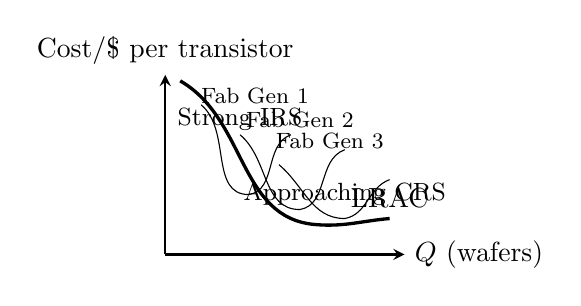
\begin{tikzpicture}[scale=0.38, thick, >=stealth]
    \draw[->] (0,0) -- (8,0) node[right] {$Q$ (wafers)};
    \draw[->] (0,0) -- (0,6) node[above] {Cost/\$ per transistor};
    % LRAC curve: steeply falling, then flat
    \draw[very thick] (0.5,5.8) to[out=330,in=175] (5,1) to[out=355,in=185] (7.5,1.2) node[above] {LRAC};
    \node at (2.5,4.5) {\small Strong IRS};
    \node at (6,2) {\small Approaching CRS};
    % SRAC curves
    \draw[thin] (1.2,5) to[out=320,in=180] (2.8,2) to[out=10,in=200] (4.2,4);
    \draw[thin] (2.5,4) to[out=320,in=180] (4.5,1.5) to[out=10,in=200] (6,3.5);
    \draw[thin] (3.8,3) to[out=320,in=180] (6,1.2) to[out=10,in=200] (7.5,2.5);
    \node at (3,5.3) {\footnotesize Fab Gen 1};
    \node at (4.5,4.5) {\footnotesize Fab Gen 2};
    \node at (5.5,3.8) {\footnotesize Fab Gen 3};
\end{tikzpicture}
\end{center}
\textit{Each SRAC represents a generation of fab technology. LRAC is the envelope, falling steeply then flattening as diminishing returns to scale (managerial complexity) offset technical economies.}

\textbf{Economic Lessons:}
\begin{enumerate}[leftmargin=*,nosep]
    \item \textbf{Returns to scale} are the central competitive dynamic in capital-intensive industries. The firm with larger scale has lower ATC and can underprice rivals.
    \item \textbf{Learning curves} and fixed R\&D amortization are critical sources of increasing returns to scale.
    \item \textbf{The SR vs. LR distinction:} Short-run capacity constraints (diminishing returns within a fab) create business cycle dynamics (chip shortages). Long-run expansion (new fabs) involves strategic scale decisions.
    \item Government industrial policy (CHIPS Act) recognizes the public-good and national-security externality of having domestic scale in semiconductor production, given massive economies of scale.
\end{enumerate}

% ============================================================================
% PART 7: EXAM QUESTIONS
% ============================================================================
\section*{7. Exam Practice Questions \& Model Answers}

\subsection*{Question 1: Calculating Products and Costs}
\textbf{Firm's production function: $Q = 2L^{0.5}$, where $Q$ is output and $L$ is labor. Wage rate $w = \$20$.}
\textbf{(a) Derive $TP_L$, $AP_L$, and $MP_L$ for $L = 1, 4, 9, 16$.}
\textbf{(b) At what $L$ does diminishing returns set in?}
\textbf{(c) Find $TVC$, $AVC$, and $MC$ as functions of $Q$.}
\textbf{(d) Show that $MC = w / MP_L$.}

\vspace{0.1cm}
\textbf{Solution:}
\vspace{0.05cm}
\textbf{(a)}
\begin{tabular}{@{}c|c|c|c@{}}
\hline $L$ & $Q = 2L^{0.5}$ & $AP_L = Q/L$ & $MP_L = dQ/dL = L^{-0.5}$ \\
\hline 1 & 2.00 & 2.00 & 1.00 \\
4 & 4.00 & 1.00 & 0.50 \\
9 & 6.00 & 0.67 & 0.33 \\
16 & 8.00 & 0.50 & 0.25 \\
\hline
\end{tabular}

\textbf{(b)} $MP_L = L^{-0.5}$. $d(MP_L)/dL = -0.5 L^{-1.5} < 0$ for all $L>0$. \textbf{Diminishing returns set in immediately} from the first unit of labor. (This function has diminishing MP throughout.)

\textbf{(c)} $Q = 2L^{0.5} \Rightarrow L = Q^2/4$. $TVC = wL = 20 \cdot (Q^2/4) = 5Q^2$.
$AVC = TVC/Q = 5Q$. $MC = d(TVC)/dQ = 10Q$.

\textbf{(d)} $MP_L = L^{-0.5} = (Q^2/4)^{-0.5} = 2/Q$. $w/MP_L = 20 / (2/Q) = 10Q = MC$. Verified. $\checkmark$

\vspace{0.2cm}

\subsection*{Question 2: Short-Run and Long-Run Costs}
\textbf{A firm's production is $Q = \sqrt{LK}$. In the short run, $K = 16$. $w = 4$, $r = 1$.}
\textbf{(a) Derive SR cost functions: TC(Q), ATC(Q), MC(Q).}
\textbf{(b) In the long run, find the cost-minimizing $L$ and $K$ for a given $Q$, and the LR cost function $C(Q)$.}
\textbf{(c) Compare SR and LR ATC for $Q = 4$, $Q = 8$, $Q = 16$. Explain differences.}

\vspace{0.05cm}
\textbf{Solution:}
\vspace{0.05cm}
\textbf{(a)} SR: $K=16$. $Q = \sqrt{L \cdot 16} = 4\sqrt{L} \Rightarrow L = Q^2/16$.
$TC = wL + rK = 4(Q^2/16) + 1(16) = Q^2/4 + 16$.
$ATC = Q/4 + 16/Q$. $MC = Q/2$.

\textbf{(b)} LR: $MRTS = MP_L/MP_K = \frac{0.5 K^{0.5} L^{-0.5}}{0.5 L^{0.5} K^{-0.5}} = K/L$. Set $K/L = w/r = 4 \Rightarrow K = 4L$.
Output: $Q = \sqrt{L \cdot 4L} = \sqrt{4L^2} = 2L \Rightarrow L = Q/2$, $K = 4(Q/2) = 2Q$.
$C(Q) = 4(Q/2) + 1(2Q) = 2Q + 2Q = 4Q$.
$LRAC = 4$, $LRMC = 4$ (constant returns to scale).

\textbf{(c)}
\begin{itemize}[nosep]
    \item $Q=4$: SR ATC = $4/4 + 16/4 = 1+4 = 5$. LR AC = $4$. SR cost higher (overcapitalized).
    \item $Q=8$: SR ATC = $8/4 + 16/8 = 2+2 = 4$. LR AC = $4$. SR = LR (\textbf{tangency point}: $K=16$ is optimal for $Q=8$).
    \item $Q=16$: SR ATC = $16/4 + 16/16 = 4+1 = 5$. LR AC = $4$. SR cost higher (undercapitalized for larger $Q$).
\end{itemize}

\vspace{0.2cm}

\subsection*{Question 3: Conceptual Comparison}
\textbf{Distinguish clearly between the ``Law of Diminishing Returns'' and ``Decreasing Returns to Scale.'' Provide real-world examples.}

\vspace{0.05cm}
\textbf{Answer:}
\begin{center}
\begin{tabular}{@{}p{2.8cm}p{3cm}p{3cm}@{}}
\toprule
\textbf{Feature} & \textbf{Diminishing Returns} & \textbf{Decreasing Returns to Scale} \\
\midrule
Time Horizon & \textbf{Short Run} (at least one fixed factor) & \textbf{Long Run} (all factors variable) \\
Cause & Adding variable input to fixed input $\to$ congestion & Increasing all inputs proportionately $\to$ output rises less than proportionately \\
Reason & Overcrowding, inefficiency with fixed capacity & Management complexity, coordination problems, bureaucracy \\
Example & Adding more workers to a fixed-size office reduces per-worker output & A startup that grows into a multinational faces communication breakdowns and slower growth \\
\bottomrule
\end{tabular}
\end{center}
\textit{Analogy:} Diminishing returns is like adding more chefs to a fixed kitchen; decreasing returns to scale is like trying to run a global restaurant chain and struggling with management.

\vspace{0.2cm}

\subsection*{Question 4: Application/Graphical}
\textbf{Draw and explain the relationship between MP, AP, MC, and AVC curves. Why does MC intersect AVC at the minimum of AVC?}

\vspace{0.05cm}
\textbf{Answer:} (Provide description and graph). The relationship stems from the duality $AVC = w/AP_L$ and $MC = w/MP_L$. When $AP_L$ is maximum, $AVC$ is minimum. When $MP_L = AP_L$ (intersection at max AP), $MC = AVC$ (intersection at min AVC). The ``average-marginal relationship'' in mathematics dictates: if the marginal is below the average, the average falls; if above, it rises. Thus, $MC$ must equal $AVC$ exactly at the minimum point of $AVC$. The same logic applies for $ATC$.

\end{multicols}

% ============================================================================
% SUMMARY TABLE
% ============================================================================
\vspace{0.3cm}
\begin{center}
\fbox{\begin{minipage}{0.9\textwidth}
\footnotesize
\textbf{Summary Cheat Sheet: Production and Cost}
\begin{center}
\begin{tabular}{@{}p{3cm}p{2.8cm}p{3.2cm}@{}}
\toprule
\textbf{Concept} & \textbf{Formula} & \textbf{Key Insight} \\
\midrule
Production Function & $Q = f(L, K)$ & Maximum output from given inputs \\
Marginal Product & $MP_L = \partial Q/\partial L$ & Extra output from one more unit of labor \\
Average Product & $AP_L = Q/L$ & Output per worker; productivity \\
Diminishing Returns (SR) & $\partial MP_L/\partial L < 0$ & Variable factor on fixed factor $\to$ MP eventually falls \\
Returns to Scale (LR) & $f(\lambda L, \lambda K) \text{ vs. } \lambda Q$ & IRS/CRS/DRS depending on proportional output response \\
$TC = TFC + TVC$ & Sum of fixed and variable costs & TFC independent of Q; TVC rises with Q \\
$MC = dTC/dQ$ & $= w/MP_L$ & Inverse of MP; U-shaped \\
$ATC = AFC + AVC$ & $= TC/Q$ & U-shaped; envelope of AVC and AFC \\
$MC$ cuts $AVC$, $ATC$ & At their minimum points & Mathematical necessity: marginal pulls average \\
LRAC & Envelope of SRACs & Firm chooses optimal plant size for each Q \\
\bottomrule
\end{tabular}
\end{center}

\vspace{0.1cm}
\textbf{Quick Check: Cost Curve Shapes and Causes}
\begin{itemize}[leftmargin=*,nosep]
    \item \textbf{U-shape of MC:} Initially falls due to specialization/returns; rises due to diminishing returns.
    \item \textbf{U-shape of AVC/ATC:} Driven by MC. MC below $\to$ AVC falls; MC above $\to$ AVC rises.
    \item \textbf{AFC falls continuously:} ``Spreading overhead'' -- TFC divided by increasing Q.
    \item \textbf{LRAC U-shape:} Economies of scale (falling), then diseconomies (rising).
\end{itemize}
\end{minipage}}
\end{center}

\end{document}